\documentclass{beamer}
\usepackage{ctex}
\usetheme{SimplePlus}
\setbeamertemplate{footline}{}

\usepackage{tikz}
\usetikzlibrary{arrows.meta}
\usepackage{tikz-cd}

\usepackage{unicode-math}
%\setmathfont{STIX Two Math}
%\setmathfont{TeX Gyre Termes Math}
%\setmathfont{Libertinus Math}
%\setmathfont{Fira Math}

%%%%%%%% FONT TIMESAVES %%%%%%%
\newcommand{\bT}{\mathbb{T}}
\newcommand{\bN}{\mathbb{N}}
\newcommand{\bI}{\mathbb{I}}

\newcommand{\CC}{\mathcal{C}}

%%%%%%%% CATEGORY THEORY %%%%%%%
\newcommand{\id}{\mathrm{id}}
\DeclareMathOperator{\Hom}{Hom}

\newcommand{\cat}[1]{\mathrm{#1}}
\newcommand{\Set}{\cat{Set}}

\DeclareFontFamily{U}{dmjhira}{}
\DeclareFontShape{U}{dmjhira}{m}{n}{ <-> dmjhira }{}

\DeclareRobustCommand{\yo}{\text{\usefont{U}{dmjhira}{m}{n}\symbol{"48}}}

\DeclareMathOperator*{\colim}{colim}

\newcommand{\inl}{\operatorname{inl}}
\newcommand{\inr}{\operatorname{inr}}

%%%%%%%%% GEOMTERY %%%%%%%%%%%%%%
\newcommand{\Spec}{\operatorname{Spec}}
\newcommand{\Zar}{\mathrm{Zar}}

%%%%%%%%% TYPE THEORY %%%%%%%%%%%
\newcommand{\OO}{\bigcirc}
\newcommand{\UU}{\mathcal{U}}
\newcommand{\isEquiv}{\bibopenparen{isEquiv}}
\newcommand{\hlevel}{\mathrm{hlevel}}
\newcommand{\isContr}{\operatorname{isContr}}
\newcommand{\isProp}{\operatorname{isProp}}
\newcommand{\Prop}{\mathrm{Prop}}
\newcommand{\refl}{\mathrm{refl}}
\newcommand{\isModal}{\operatorname{isModal}}
\newcommand{\ap}{\operatorname{ap}}
\newcommand{\fib}{\operatorname{fib}}
\newcommand{\im}{\operatorname{im}}
\newcommand{\tot}{\mathrm{tot}}
\newcommand{\pt}{\mathrm{pt}}

\title{sketch}

\date{}

\begin{document}

\begin{frame}
    % Print the title page as the first slide
    \titlepage
\end{frame}

\begin{frame}{Motivation\cite{makkai_pare}}
Roughly speaking, a sketch is a presentation of a category with certain prescribed limits and colimits. Because of the expressibility of certain logical operations by limits and colimits (see below), sketches can be used as presentations of theories. The point of view of considering sketches as theories is present throughout the literature on sketches; see e.g. R. Guitart and C. Lair [G/L] and the recent book [B/W] by M. Barr and C. Wells.
\end{frame}

\begin{frame}{图(graph)}
A \textbf{graph} $G$ consists of two sets $G_0$ and $G_1$ and two functions $\operatorname{source}\colon G_1 \to G_0$ and $\operatorname{target}\colon G_1 \to G_0$.

\vspace{6mm}

The elements of $G_0$ are called the \textbf{nodes} or \textbf{vertices} of $G$ and the elements of $G_1$ are the \textbf{arrows} of $G$. If an arrow $a$ has source $x$ and target $y$ we write $a\colon x \to y$. A graph is conventionally drawn using dots or labels for the nodes, and an arrow going from node $x$ to node $y$ for each element $a$ of $G_1$ with source $x$ and target $y$.
\end{frame}

\begin{frame}[fragile]{图同态(homomorphism of graphs)}
A \textbf{homomorphism of graphs} $f\colon G \to H$ is a pair of functions $f_0\colon G_0 \to H_0$ and $f_1\colon G_1 \to H_1$ for which these diagrams commute:
\[
\begin{tikzcd}[column sep=large,row sep=large]
G_1 \arrow[r,"f_1"] \arrow[d,"\operatorname{source}"'] & H_1 \arrow[d,"\operatorname{source}"] \\
G_0 \arrow[r,"f_0"'] & H_0
\end{tikzcd}
\qquad\quad
\begin{tikzcd}[column sep=large,row sep=large]
G_1 \arrow[r,"f_1"] \arrow[d,"\operatorname{target}"'] & H_1 \arrow[d,"\operatorname{target}"] \\
G_0 \arrow[r,"f_0"'] & H_0
\end{tikzcd}
\]

\vspace{5mm}

Every category has an \textbf{underlying graph} whose nodes are the objects of the category and whose arrows are the arrows of the category with the same source and target.
\end{frame}

\begin{frame}[fragile]{自然变换(natural transformation)}
Let $f,f'\colon G \to \mathcal{C}$ be graph homomorphisms to a category $\mathcal{C}$. A \textbf{natural transformation} $\phi\colon f \to f'$ is a family of arrows $\phi_x\colon f(x) \to f'(x)$ indexed by the nodes of $G$ with the property that for every arrow $u\colon x \to x'$ of $G$ the following diagram commutes:
\[
\begin{tikzcd}
f(x) \arrow[r,"\phi_x"] \arrow[d,"f(u)"'] & f'(x) \arrow[d,"f'(u)"] \\
f(x') \arrow[r,"\phi_{x'}"'] & f'(x')
\end{tikzcd}
\]
\end{frame}

\begin{frame}{路径(path)}
A \textbf{path} of length $n$ from $x$ to $y$ in a graph $G$ is a sequence $\langle f_1,f_2,\dots,f_n\rangle$ of arrows with the property that the target of $f_{j-1}$ is the source of $f_j$ for $j=2,\dots,n$, $\operatorname{source}(f_1)=x$ and $\operatorname{target}(f_n)=y$. If $p=\langle f_1,f_2,\dots,f_n\rangle$ is a path from $x$ to $y$, we write $p\colon x \to y$. For each node $x$, there is one \textbf{empty path} $\langle\rangle\colon x \to x$.

\vspace{2mm}

We extend the definition of homomorphism $F\colon G \to H$ of graphs to paths in $G$ by mapping $F$ over the nodes in the path:
\[
F\langle f_1,f_2,\dots,f_n\rangle = \langle F(f_1),F(f_2),\dots,F(f_n)\rangle
\]

The nodes of $G$ and the paths form a category, the \textbf{free category} generated by the graph $G$, with the empty paths as identity arrows and composition by concatenation.

\vspace{2mm}

The set of paths of length $n$ in $G$ is denoted $G_n$. In particular, a path of length $2$ is a pair $\langle f,g\rangle$ of arrows such that the source of $g$ is the target of $f$. Such a pair is called a \textbf{composable pair}.
\end{frame}

\begin{frame}[fragile]{自反图(Reflexive Graph)}
A \textbf{reflexive graph} is a graph with additional structure, namely a function $\operatorname{loop}\colon G_0 \to G_1$ satisfying the equations
\[
\begin{tikzcd}
G_0 \arrow[r, "\operatorname{loop}"] \arrow[dr, "G_0"'] & G_1 \arrow[d, "\operatorname{source}"] \\
& G_0
\end{tikzcd}
\qquad
\begin{tikzcd}
G_0 \arrow[r, "\operatorname{loop}"] \arrow[dr, "G_0"'] & G_1 \arrow[d, "\operatorname{target}"] \\
& G_0
\end{tikzcd}
\]

\vspace{2mm}

(In this text, I follow the categorial custom of using the name of an object also as the name of its identity arrow.) The arrows of the form $\operatorname{loop}(x)$ for some node $x$ are called the \textbf{distinguished loops}.

\vspace{2mm}

A \textbf{homomorphism of reflexive graphs} is a homomorphism of graphs that takes distinguished loops to distinguished loops.

\vspace{2mm}

The \textbf{underlying reflexive graph} of a category is the underlying graph with the identity arrows as the distinguished loops.
\end{frame}

\begin{frame}[fragile,shrink]{可复合图(Compositive graphs)}
The French school bases its definition of sketch on the concept of a \textbf{compositive graph} or \textbf{multiplicative graph}: A compositive graph $G$ is a reflexive graph with a partially defined binary operation $\kappa\colon C_G \to G$ satisfying the laws CG.1 through CG.3 below. If $\langle f,g\rangle$ is a composable pair and $\kappa(f,g)$ is defined, we write $g\circ f$ for $\kappa(f,g)$ (note the reversal).

\noindent\textbf{CG.1}\quad $C_G$ is a subset of $G_2$.

\noindent\textbf{CG.2}\quad For all arrows $f$, $f\circ \operatorname{id}_{\operatorname{source}(f)}$ and $\operatorname{id}_{\operatorname{target}(f)}\circ f$ are both defined and equal to $f$.

\noindent\textbf{CG.3}\quad If $g\circ f$ is defined, $\operatorname{source}(g\circ f) = \operatorname{source}(f)$ and $\operatorname{target}(g\circ f) = \operatorname{target}(g)$.

\medskip

Associativity is not required. A \textbf{category} is a compositive graph $G$ for which $C_G = G_2$ and the composition is associative.

A \textbf{functor} between compositive graphs is defined just like functors between categories. In all cases, if $F$ is a functor and $g\circ f$ is defined, then $F(g)\circ F(f)$ is defined and equal to $F(g\circ f)$.
\end{frame}

\begin{frame}{图表(Diagrams)}
If $I$ and $G$ are graphs, a graph homomorphism $d\colon I \to G$ is a \textbf{diagram} in $G$. In this case, $I$ is the \textbf{shape graph} of the diagram. If $I$ is a graph, $\mathcal{C}$ is a category, and $d$ is a diagram in the underlying graph of $\mathcal{C}$, we will write it as $d\colon I \to \mathcal{C}$.
\end{frame}

\begin{frame}[fragile]
By convention, a diagram is drawn in such a way that its shape graph can be recovered (except for the actual names of the nodes and arrows) from the way it is drawn by replacing each node of the drawn graph by a different label (whether two nodes as drawn have the same label or not) and similarly for arrows. For example, the shape graphs corresponding to these two diagrams
\begin{equation}\label{eq:diagrams}
\begin{minipage}[t]{0.45\textwidth}
\centering
\begin{tikzcd}
G \arrow[r, "f"] \arrow[dr, "h"'] & H \arrow[d, "g"] \\
& G
\end{tikzcd}
\end{minipage}
\hfill
\begin{minipage}[t]{0.45\textwidth}
\centering
\begin{tikzcd}
G \arrow[loop above, "h"] \arrow[r, shift left, "f"] & H \arrow[l, shift left, "g"]
\end{tikzcd}
\end{minipage}
\end{equation}
are these two graphs respectively:
\[
\begin{minipage}[t]{0.45\textwidth}
\centering
\begin{tikzcd}
i \arrow[r, "a"] \arrow[dr, "b"'] & j \arrow[d, "c"] \\
& k
\end{tikzcd}
\end{minipage}
\hfill
\begin{minipage}[t]{0.45\textwidth}
\centering
\begin{tikzcd}
u \arrow[loop above, "b"] \arrow[r, shift left, "a"] & v \arrow[l, shift left, "c"]
\end{tikzcd}
\end{minipage}
\]

The diagrams in \eqref{eq:diagrams} are not the same!
\end{frame}

\begin{frame}
A diagram $d\colon I \to \mathcal{C}$ in a category $\mathcal{C}$ is \textbf{commutative} if for all pairs of paths $p,q\colon x \to y$ in the shape graph $I$ between the same two nodes, $d(p)$ and $d(q)$ have the same composites in $\mathcal{C}$. For example, if the left diagram in \eqref{eq:diagrams} commutes, then $g\circ f = h$, whereas if the right diagram commutes, then $g\circ f = h = \operatorname{id}_G$ and $f\circ g = \operatorname{id}_H$. (The point is that there is an empty path from $G$ to $G$ and another one from $H$ to $H$.)

The concept of commutative diagram requires composition; it makes sense in a compositive graph but not in a graph in general.

In much of the categorial literature, a diagram $d\colon I \to \mathcal{C}$ is defined to be a functor from a category (most commonly a small category) $I$ to $\mathcal{C}$. A graph-based diagram can be converted to an equivalent category-based one by basing it on the free category generated by the graph. Conversely, a functor defined on a category $\mathcal{I}$ is a diagram based on the underlying graph of $\mathcal{I}$. But be careful: there are in general diagrams based on the underlying graph of $\mathcal{I}$ that are not functors from $\mathcal{I}$, because there is no way to enforce the preservation of composition. (自由范畴 $F(U(\mathcal{I}))$ 并不等于原始范畴 $\mathcal{I}$)
\end{frame}

\begin{frame}[fragile,shrink]{锥(Cones)}
If $d\colon I \to G$ is a diagram in a graph $G$, then a \textbf{cone} $p\colon v \to d$ consists of an object $v$ of $G$ and a set of arrows $p_k\colon v \to d(k)$ indexed by the nodes of $I$. If $d\colon I \to \mathcal{C}$ is a diagram in a category $\mathcal{C}$, the cone $p\colon v \to d$ is \textbf{commutative} if for all arrows $u\colon k \to k'$ in $I$,
\[
\begin{tikzcd}
v \arrow[r, "p_k"] \arrow[dr, "p_{k'}"'] & d(k) \arrow[d, "d(u)"] \\
& d(k')
\end{tikzcd}
\]
commutes.

The diagram $d$ is called the \textbf{base diagram} of the cone and the arrows $p_k$ are the \textbf{projections} or sometimes \textbf{elements} of the cone.

Note that the concept of commutative cone does not make sense for a cone in a graph, although it does for a cone in a compositive graph. For most authors, a cone in a compositive graph (hence in a category) is commutative by definition.

The base diagram of a cone in a category is \emph{not required to be commutative}.

If the shape graph of the base diagram has only identity arrows, the cone is \textbf{discrete}.
\end{frame}

\begin{frame}[fragile]{余锥(cocone)}
A \textbf{cocone} in $\mathcal{C}$ based on a diagram $d\colon I \to \mathcal{C}$ consists of an object $v$ of $\mathcal{C}$ and arrows $i_k\colon d(k) \to v$ indexed by the objects of $I$. It is commutative if for all $u\colon k \to k'$ in $I$,
\[
\begin{tikzcd}
v & d(k) \arrow[l, "i_k"'] \arrow[d, "d(u)"] \\
& d(k') \arrow[ul, "i_{k'}"]
\end{tikzcd}
\]
commute.
\end{frame}

\begin{frame}{草图(sketch)}
A \textbf{sketch} $\mathsf{S}$ consists of a graph $G_{\mathsf{S}}$, a set $D_{\mathsf{S}}$ of diagrams in $G_{\mathsf{S}}$, a set $L_{\mathsf{S}}$ of cones in $G_{\mathsf{S}}$ and a set $C_{\mathsf{S}}$ of cocones in $G_{\mathsf{S}}$.
\end{frame}

\begin{frame}{草图的态射(Morphisms of sketches)}
If $\mathsf{S}$ and $\mathsf{S}'$ are sketches, a graph homomorphism $f\colon G_{\mathsf{S}} \to G_{\mathsf{S}'}$ is a \textbf{morphism of sketches} if it takes each diagram of $\mathsf{S}$ to a diagram of $\mathsf{S}'$, each cone of $\mathsf{S}$ to a cone of $\mathsf{S}'$, and each cocone of $\mathsf{S}$ to a cocone of $\mathsf{S}'$. This produces the category $\mathbf{\mathsf{Sk}}$ of sketches.

\bigskip

Each small category $\mathcal{C}$ has an \textbf{underlying sketch} whose graph is the underlying graph of $\mathcal{C}$, whose diagrams are all the \textcolor{red}{commutative} diagrams in $\mathcal{C}$, whose cones are all the limit cones in $\mathcal{C}$ and whose cocones are all the colimit cocones in $\mathcal{C}$.
\end{frame}

\begin{frame}{草图的模型(Models of sketches)}
Let $\mathsf{S}$ be a sketch and $\mathcal{C}$ a category. $M\colon \mathsf{S} \to \mathcal{C}$ is a \textbf{model of $\mathsf{S}$ in $\mathcal{C}$} if $M$ is a sketch morphism from $\mathsf{S}$ to the underlying sketch of $\mathcal{C}$. If $M$ and $M'$ are two models of $\mathsf{S}$ in $\mathcal{C}$, $\mu\colon M \to M'$ is a \textbf{homomorphism of models} if $\mu$ is a natural transformation from $M$ to $M'$.

\bigskip

This produces a \textbf{category of models of the sketch $\mathsf{S}$ in $\mathcal{C}$}, using vertical composition of natural transformations as the composition.

This category is denoted $\operatorname{Mod}_{\mathcal{C}}(\mathsf{S})$. The category of models of $\mathsf{S}$ in the category of sets is denoted $\operatorname{Mod}(\mathsf{S})$, and normally the phrase ``model of $\mathsf{S}$'' without qualification means a model in the category of sets.
\end{frame}

\begin{frame}
A model of a sketch in the category of sets associates a set with each node of the graph of the sketch, so that the nodes of the graph specify the \emph{sorts} of the structure. The arrows correspond to mappings between sets that are values of the sorts, so they specify the \emph{operations} of the structure. The cones and cocones formally specify \emph{constructed sorts}. For example, a discrete cone whose diagram has $n$ nodes specifies a set of $n$-tuples, with the $i$th entry drawn from the value of the $i$th node in the diagram. General limit diagrams specify equationally defined subsorts, and colimit diagrams specify quotient structures (coequalizers), free products (coproducts), and amalgamated products (pushouts).
\end{frame}

\begin{frame}[fragile,shrink]
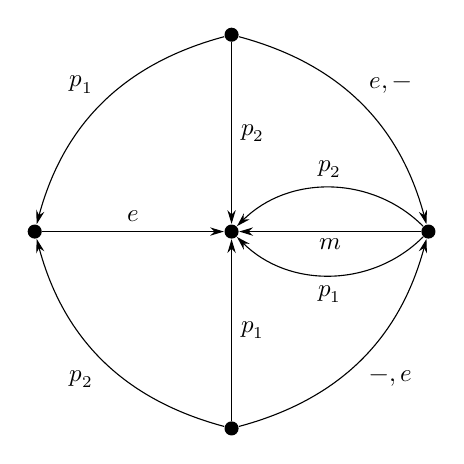
\begin{tikzpicture}[
    dot/.style={circle, fill=black, inner sep=1.8pt},
    >={Stealth[length=5pt, width=3pt]},
    node distance=2.5cm,
    font=\small
]
    % 节点定义 (5个顶点)
    \node[dot] (L) at (-2.5, 0) {};  % 左节点
    \node[dot] (C) at (0, 0) {};     % 中心节点
    \node[dot] (R) at (2.5, 0) {};   % 右节点
    \node[dot] (T) at (0, 2.5) {};   % 上节点
    \node[dot] (B) at (0, -2.5) {};  % 下节点

    % --- 左边到中心的边 ---
    \draw[->] (L) -- node[above] {$e$} (C);

    % --- 上节点出发的边 ---
    \draw[->] (T) to[bend right=30] node[above left] {$p_1$} (L);
    \draw[->] (T) -- node[right] {$p_2$} (C);
    \draw[->] (T) to[bend left=30] node[above right] {$e,-$} (R);

    % --- 下节点出发的边 ---
    \draw[->] (B) to[bend left=30] node[below left] {$p_2$} (L);
    \draw[->] (B) -- node[right] {$p_1$} (C);
    \draw[->] (B) to[bend right=30] node[below right] {$-,e$} (R);

    % --- 右节点到中心节点的 3 条平行/弯曲边 ---
    \draw[->] (R) to[bend right=45] node[above] {$p_2$} (C);
    \draw[->] (R) -- node[below=-1pt] {$m$} (C);
    \draw[->] (R) to[bend left=45] node[below] {$p_1$} (C);

\end{tikzpicture}

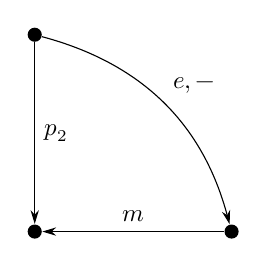
\begin{tikzpicture}[
    dot/.style={circle, fill=black, inner sep=1.8pt},
    >={Stealth[length=5pt, width=3pt]},
    node distance=2.5cm,
    font=\small
]
    % 节点定义 (3个顶点)
    \node[dot] (T) at (0, 2.5) {};   % 上节点
    \node[dot] (C) at (0, 0) {};     % 左下节点
    \node[dot] (R) at (2.5, 0) {};   % 右下节点

    % 1. 从上节点指向左下节点的直线
    \draw[->] (T) -- node[right] {$p_2$} (C);

    % 2. 从右下节点指向左下节点的直线
    \draw[->] (R) -- node[above] {$m$} (C);

    % 3. 从上节点指向右下节点的弯曲弧线
    \draw[->] (T) to[bend left=30] node[above right] {$e,-$} (R);

\end{tikzpicture}
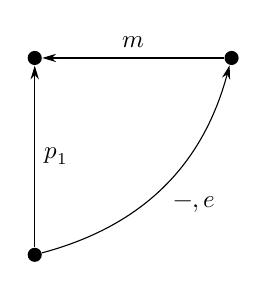
\begin{tikzpicture}[
    dot/.style={circle, fill=black, inner sep=1.8pt},
    >={Stealth[length=5pt, width=3pt]},
    node distance=2.5cm,
    font=\small
]
    % 节点定义 (3个顶点)
    \node[dot] (BL) at (0, 0) {};     % 左下节点
    \node[dot] (TL) at (0, 2.5) {};   % 左上节点
    \node[dot] (TR) at (2.5, 2.5) {}; % 右上节点

    % 1. 从左下节点指向左上节点的直线
    \draw[->] (BL) -- node[right] {$p_1$} (TL);

    % 2. 从右上节点指向左上节点的直线
    \draw[->] (TR) -- node[above] {$m$} (TL);

    % 3. 从左下节点指向右上节点的弯曲弧线
    \draw[->] (BL) to[bend right=30] node[below right] {$-,e$} (TR);

\end{tikzpicture}
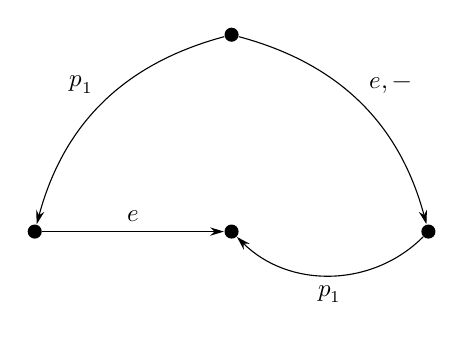
\begin{tikzpicture}[
    dot/.style={circle, fill=black, inner sep=1.8pt},
    >={Stealth[length=5pt, width=3pt]},
    node distance=2.5cm,
    font=\small
]
    % 节点定义 (4个顶点)
    \node[dot] (L) at (-2.5, 0) {};   % 左节点
    \node[dot] (C) at (0, 0) {};      % 中心节点
    \node[dot] (R) at (2.5, 0) {};    % 右节点
    \node[dot] (T) at (0, 2.5) {};    % 上节点

    % 1. 左节点指向中心节点的直线
    \draw[->] (L) -- node[above] {$e$} (C);

    % 2. 上节点指向左节点的弯曲弧线
    \draw[->] (T) to[bend right=30] node[above left] {$p_1$} (L);

    % 3. 上节点指向右节点的弯曲弧线
    \draw[->] (T) to[bend left=30] node[above right] {$e,-$} (R);

    % 4. 右节点指向中心节点的下弯弧线
    \draw[->] (R) to[bend left=45] node[below] {$p_1$} (C);

\end{tikzpicture}
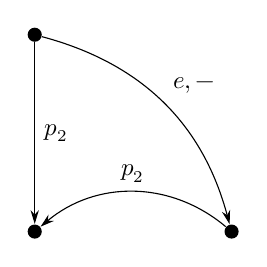
\begin{tikzpicture}[
    dot/.style={circle, fill=black, inner sep=1.8pt},
    >={Stealth[length=5pt, width=3pt]},
    node distance=2.5cm,
    font=\small
]
    % 节点定义 (3个顶点)
    \node[dot] (TL) at (0, 2.5) {};   % 左上节点
    \node[dot] (BL) at (0, 0) {};     % 左下节点
    \node[dot] (BR) at (2.5, 0) {};   % 右下节点

    % 1. 从左上节点指向左下节点的直线
    \draw[->] (TL) -- node[right] {$p_2$} (BL);

    % 2. 从右下节点指向左下节点的弯曲弧线
    \draw[->] (BR) to[bend right=40] node[above] {$p_2$} (BL);

    % 3. 从左上节点指向右下节点的弯曲弧线
    \draw[->] (TL) to[bend left=30] node[above right] {$e,-$} (BR);

\end{tikzpicture}
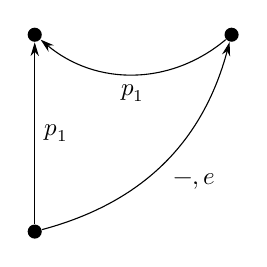
\begin{tikzpicture}[
    dot/.style={circle, fill=black, inner sep=1.8pt},
    >={Stealth[length=5pt, width=3pt]},
    node distance=2.5cm,
    font=\small
]
    % 节点定义 (3个顶点)
    \node[dot] (BL) at (0, 0) {};     % 左下节点
    \node[dot] (TL) at (0, 2.5) {};   % 左上节点
    \node[dot] (TR) at (2.5, 2.5) {}; % 右上节点

    % 1. 从左下节点指向左上节点的直线
    \draw[->] (BL) -- node[right] {$p_1$} (TL);

    % 2. 从右上节点指向左上节点的弯曲弧线
    \draw[->] (TR) to[bend left=40] node[below] {$p_1$} (TL);

    % 3. 从左下节点指向右上节点的弯曲弧线
    \draw[->] (BL) to[bend right=30] node[below right] {$-, e$} (TR);

\end{tikzpicture}
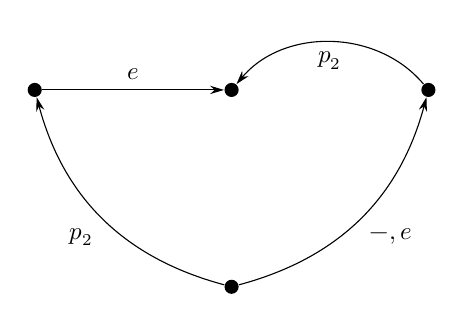
\begin{tikzpicture}[
    dot/.style={circle, fill=black, inner sep=1.8pt},
    >={Stealth[length=5pt, width=3pt]},
    font=\small
]
    % 节点定义 (4个顶点)
    \node[dot] (TL) at (0, 2.5) {};   % 左上节点
    \node[dot] (TM) at (2.5, 2.5) {}; % 中上节点
    \node[dot] (TR) at (5.0, 2.5) {}; % 右上节点
    \node[dot] (BM) at (2.5, 0) {};   % 中下节点

    % 1. 从左上节点指向中上节点的直线箭头
    \draw[->] (TL) -- node[above] {$e$} (TM);

    % 2. 从右上节点指向中上节点的弯曲弧线
    \draw[->] (TR) to[bend right=50] node[below] {$p_2$} (TM);

    % 3. 从中下节点指向左上节点的弯曲弧线
    \draw[->] (BM) to[bend left=30] node[below left] {$p_2$} (TL);

    % 4. 从中下节点指向右上节点的弯曲弧线
    \draw[->] (BM) to[bend right=30] node[below right] {$-, e$} (TR);

\end{tikzpicture}
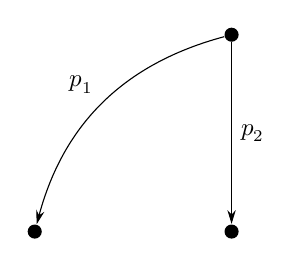
\begin{tikzpicture}[
    dot/.style={circle, fill=black, inner sep=1.8pt},
    >={Stealth[length=5pt, width=3pt]},
    font=\small
]
    % 节点定义 (3个顶点)
    \node[dot] (BL) at (0, 0) {};     % 左下节点
    \node[dot] (BR) at (2.5, 0) {};   % 右下节点
    \node[dot] (TR) at (2.5, 2.5) {}; % 右上节点

    % 1. 从右上节点指向左下节点的弯曲弧线
    \draw[->] (TR) to[bend right=30] node[above left] {$p_1$} (BL);

    % 2. 从右上节点指向右下节点的直线
    \draw[->] (TR) -- node[right] {$p_2$} (BR);

\end{tikzpicture}
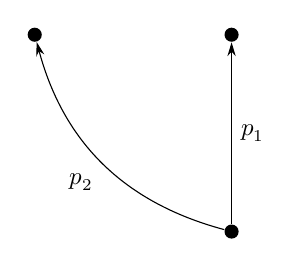
\begin{tikzpicture}[
    dot/.style={circle, fill=black, inner sep=1.8pt},
    >={Stealth[length=5pt, width=3pt]},
    font=\small
]
    % 节点定义 (3个顶点)
    \node[dot] (TL) at (0, 2.5) {};   % 左上节点
    \node[dot] (TR) at (2.5, 2.5) {}; % 右上节点
    \node[dot] (BR) at (2.5, 0) {};   % 右下节点

    % 1. 从右下节点指向右上节点的直线
    \draw[->] (BR) -- node[right] {$p_1$} (TR);

    % 2. 从右下节点指向左上节点的弯曲弧线
    \draw[->] (BR) to[bend left=30] node[below left] {$p_2$} (TL);

\end{tikzpicture}
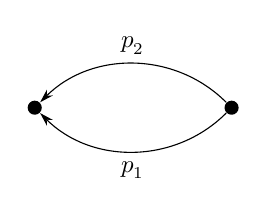
\begin{tikzpicture}[
    dot/.style={circle, fill=black, inner sep=1.8pt},
    >={Stealth[length=5pt, width=3pt]},
    font=\small
]
    % 节点定义 (2个顶点)
    \node[dot] (L) at (0, 0) {};   % 左节点
    \node[dot] (R) at (2.5, 0) {}; % 右节点

    % 1. 上方弯曲弧线 (从右指向左，标注 p_2)
    \draw[->] (R) to[bend right=45] node[above] {$p_2$} (L);

    % 2. 下方弯曲弧线 (从右指向左，标注 p_1)
    \draw[->] (R) to[bend left=45] node[below] {$p_1$} (L);

\end{tikzpicture}
\end{frame}

% 参考文献帧，长列表自动分页
\begin{frame}[allowframebreaks]{参考文献}
\begin{thebibliography}{99}

\bibitem{makkai_pare}
Michael Makkai, Robert Paré. Accessible categories: The foundations of categorical model theory.

\bibitem{wells_outline}
Charles Wells. Sketches: Outline with references, 1993

\end{thebibliography}
\end{frame}

\end{document}
